\section{OSR in LLVM}
\label{se:osr-llvm}

[...]

\ifdefined\noauthorea
\begin{figure}[t]
\begin{center}
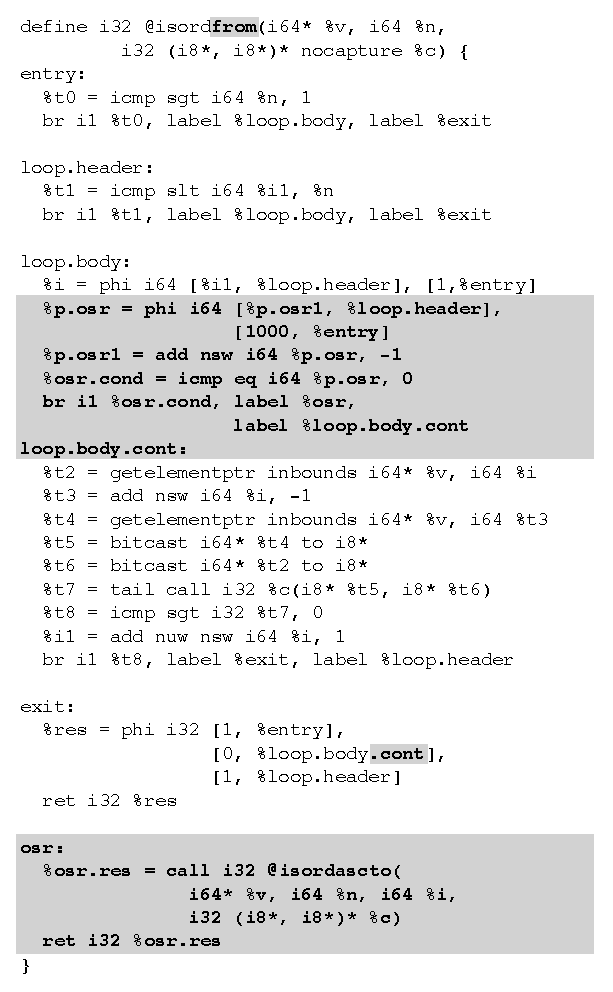
\includegraphics[width=0.9\columnwidth]{figures/isordfrom/isordfrom.eps}
\caption{\protect\label{fig:isordfrom} IR version of base function {\tt isord} (\myfigure\ref{fi:isord-example}) instrumented for resolved OSR. The OSR is fired at the beginning of the loop body after 1000 iterations. Additions resulting from the instrumentation are in grey.
}
\end{center}
\end{figure}
\fi

\ifdefined\noauthorea
\begin{figure}[t]
\begin{center}
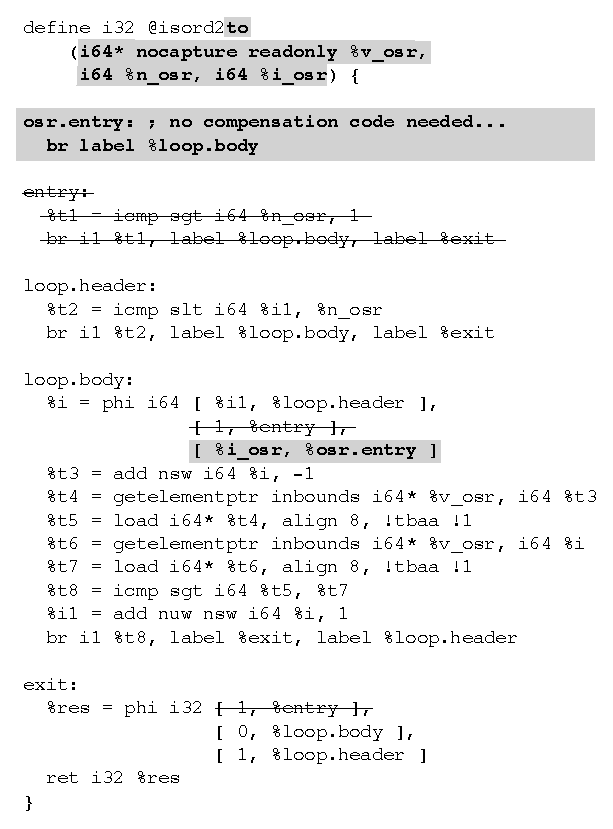
\includegraphics[width=0.9\columnwidth]{figures/isord2to/isord2to.eps}
\caption{\protect\label{fig:isordfrom} OSR instrumentation of base function in LLVM IR.
}
\end{center}
\end{figure}
\fi

\begin{verbatim}
int isord(long* v, long n, int (*c)(void* a, void* b)) {
    for (long i=1; i<n; i++) 
        if (c(v+i-1,v+i)>0) return 0;
    return 1;
}
\end{verbatim}

\begin{verbatim}
int isord2(long* v, long n) {
    for (long i=1; i<n; i++) 
        if (v[i-1]>v[i]) return 0;
    return 1;
}
\end{verbatim}

\subsection{Resolved OSR Points}

\subsection{Open OSR Points}
  
%\begin{verbatim}
%int fac(int n) {
%    int i = 2, f = 1;
%    while (i<=n) f *= i++;
%    return f;
%}
%\end{verbatim}
%
%\begin{verbatim}
%int fac(int n) {
%    int i = 2, f = 1;
%    while (i<=n)  {
%        if (osr_cond) return fac_osr(n,i,f); 
%        f *= i++; 
%    } return f;
%}
%\end{verbatim}
%
%\begin{verbatim}
%int fac_osr(int n) {
%    goto L;
%    int i = 2, f = 1;
%    while (i<=n) L: f *= i++;
%    return f;
%}
%\end{verbatim}


  
  
  
  
  